% !TEX root = saveliev_physics_general_course_2.tex
%!TEX TS-program = pdflatex
%!TEX encoding = UTF-8 Unicode

\chapter[MOVING-MEDIA OPTICS]{MOVING-MEDIA OPTICS}\label{chap:21}
\chaptermark{MOVING-MEDIA OPTICS}

\section{The Speed of Light}\label{sec:21_1}

The speed of light in a vacuum is one of the fundamental physical quantities.
The establishment of the finite nature of the speed of light had a tremendous significance of principle.
The finite nature of the speed of transmitting signals and of transmitting interactions underlies the theory of relativity.

In view of the fact that the numerical value of the speed of light is very high, the experimental determination of this speed is a very complicated task.
The speed of light was first determined on the basis of astronomical observations.
In 1676, the Danish astronomer Olaus Romer (1644-1710) determined the speed of light from observations of eclipses of Jupiter's satellites.
He obtained a value of \SI{215000}{km.s^{-1}}.

The Earth's motion in orbit results in the visible position of stars on the celestial sphere changing.
This phenomenon, called the \textbf{aberration of light}, was used in 1727 by the British astronomer James Bradley (1693-1762) to determine the speed of light.

Assume that the direction to a star seen in a telescope is perpendicular to the plane of the Earth's orbit.
Hence, the angle between the direction toward the star and the vector of the Earth's velocity $v$ will be $\pi/2$ during the entire year (\fig{21_1}).
Let us point the axis of the telescope directly at the star.
During the time $\tau$ needed for the light to cover the distance from the objective to the eyepiece, the telescope will move together with the Earth over the distance $v\tau$ in a direction at right angles to the light ray.
As a result, the image of the star will be displaced from the centre of the eyepiece.
For the image to be exactly at the centre of the eyepiece, the axis of the telescope must be turned in the direction of the vector $\vec{v}$ through the angle whose tangent is determined by the relation
\begin{equation}\label{eq:21_1}
    \tan\alpha = \frac{v}{c}
\end{equation}

(see \fig{21_1}).
In exactly the same way, raindrops falling vertically will fly through a long tube placed on a moving cart only if the axis of the tube is inclined in the direction of motion of the cart.

\begin{figure}[t]
	\begin{center}
		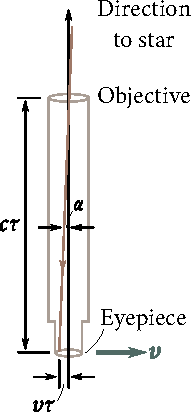
\includegraphics[scale=1]{figures/ch_21/fig_21_1.pdf}
		% \caption[]{}
        \caption[]{Bradley experimental scheme to measure the speed of light. The direction to a star seen in a telescope is perpendicular to the plane of the Earth's orbit. The angle between the direction toward the star and the vector of the Earth's velocity $v$ will be $\pi/2$ during the entire year.}
		\label{fig:21_1}
	\end{center}
	\vspace{-0.8cm}
\end{figure}

Thus, the visible position of a star is displaced relative to the true one through the angle $\alpha$.
The Earth's velocity vector constantly turns in the plane of the orbit.
Therefore, the telescope axis also turns, describing a cone about the true direction toward the star.
Accordingly, the visible position of the star on the celestial sphere describes a circle whose angular diameter is $2\alpha$.
If the direction toward the star makes an angle other than a right one with the plane of the Earth's orbit, the visible position of the star describes an ellipse whose major axis has the angular dimension $2\alpha$.
For a star in the plane of the orbit, the ellipse degenerates into a straight line.

Bradley found from astronomical observations that $2\alpha=\ang{;40.9;}$.
The corresponding value of $c$ obtained by \eqn{21_1} is \SI{303000}{km.s^{-1}}.

In terrestrial conditions, the speed of light was first measured by the French scientist Armand Fizeau (1819-1896) in 1849.
The layout of his experiment is shown in \fig{21_2}.
Light from source S fell on a half-silvered mirror.
The light reflected from the mirror got onto the edge of a rapidly rotating toothed disk.
Every time a space between the teeth was opposite the light beam, a light pulse was produced that reached mirror M and was reflected back.
If at the moment when the light returned to the disk a space was opposite the beam, the reflected pulse passed partly through the half-silvered mirror and reached the observer's eye.
If a tooth of the disk was in the path of the reflected pulse, the observer saw no light.

\begin{figure}[t]
	\begin{center}
		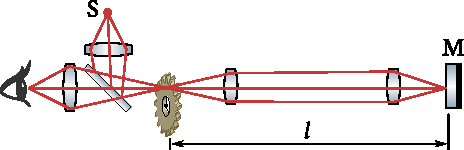
\includegraphics[scale=1]{figures/ch_21/fig_21_2.pdf}
		% \caption[]{}
        \caption[]{Fizeau experimental setup to measure the speed of light. Light from source S falls on a half-silvered mirror.
		The light reflected from the mirror hits the edge of a rapidly rotating toothed disk. Every time a space between the teeth was opposite the light beam, a light pulse was produced that reached mirror M and was reflected back. If at the moment when the light returned to the disk a space was opposite the beam, the reflected pulse passed partly through the half-silvered mirror and reached the observer's eye.
		If a tooth of the disk was in the path of the reflected pulse, the observer saw no light.}
		\label{fig:21_2}
	\end{center}
	\vspace{-0.8cm}
\end{figure}

During the time $\tau=2l/c$ needed for the light to cover the distance to mirror M and back, the disk managed to turn through the angle $\Delta{\omega}=\omega\tau=2l\omega/c$, where $\omega$ is the angular velocity of the disk.
Assume that the number of disk teeth is $N$.
Therefore, the angle between the centres of adjacent teeth is $\alpha = 2\pi/N$.
The light did not return to the observer's eye at such disk velocities at which the disk in the time $\tau$ managed to turn through the angles $\alpha/2, 3\alpha/2, \ldots, (m-1/2)\alpha$, etc.
Hence, the condition for the $m$-th blackout has the form
\begin{equation*}
	\Delta{\omega} = \parenthesis{m - \frac{1}{2}} \alpha \quad \text{or} \quad \frac{2l\omega}{c} = \parenthesis{m - \frac{1}{2}} \frac{2\pi}{N}.
\end{equation*}

\noindent
According to this formula, knowing $l$, $N$, and the angular velocity $\omega_m$ at which the $m$-th blackout is obtained, we can find $c$.
In Fizeau's experiment, $l$ was about \SI{8.6}{km}.
The value of \SI{313000}{km.s^{-1}} was obtained for $c$.

In 1928, Kerr cells (see \sect{19_7}) were used to measure the speed of light.
They made it possible to interrupt a light beam with a much higher frequency (about \SI{e7}{s^{-1}}) than when a rotating toothed disk was used.
This made measurements of $c$ possible with $l$ of the order of several metres.

Albert Michelson performed several measurements of the speed of light using the method of a rotating prism.
In Michelson's experiment conducted in 1932, light propagated in a tube \SI{1.6}{km} long from which the air was evacuated.

At present, the speed of light in a vacuum is taken equal to
\begin{equation}\label{eq:21_2}
	c = 299792.5 \pm \SI{0.1}{km.s^{-1}}.
\end{equation}

\noindent
We must note that in all the experiments in which light was interrupted, the group velocity of the light waves was determined, and not the phase velocity.
In air, these two velocities virtually coincide.

\section{Fizeau's Experiment}\label{sec:21_2}

Up to now, we assumed that the sources, receivers, and other bodies relative to which the propagation of light was considered are stationary.
It is quite natural to be interested in how motion of a source of light waves affects the propagation of light.
Here, it becomes necessary to indicate relative to what the motion takes place.
We established in \sect{14_11} that the motion of a source or a receiver of sound waves relative to the medium in which these waves are propagating affects the proceeding of acoustic phenomena (the Doppler effect), and, consequently, can be detected.

The wave theory initially treated light as elastic waves propagating in a hypothetic medium called universal ether.
After Maxwell advanced his theory, elastic ether was replaced by an ether that was a carrier of electromagnetic waves and fields.
By this ether was meant a special medium filling, like its elastic ether predecessor, the entire space of the universe and penetrating all bodies.
Since ether was a certain medium, it would be possible to count on detecting the motion of bodies, for example light sources or receivers, with respect to this medium.
In particular, the existence of an ``ether wind'' blowing around the Earth in its motion about the Sun ought to be expected.

Galileo's principle of relativity was established in mechanics.
According to it, all inertial reference frames are equivalent in a mechanical respect.
The detection of ether would make it possible to separate (with the aid of optical phenomena) a special (related to ether) predominant, absolute reference frame.
Therefore, motion of the other frames could be considered relative to this absolute frame.

Thus, the establishment of how universal ether interacts with moving bodies, was a matter of principle.
Three possibilities could be assumed: (1) ether is absolutely not disturbed by moving bodies, (2) ether is partly carried along by moving bodies, acquiring a velocity of $\alpha v$, where $v$ is the velocity of a body relative to the absolute reference frame, and $\alpha$ is a drag coefficient less than unity, and (3) ether is completely carried along by moving bodies, for example by the Earth, in the same way as a body in its motion carries along the layers of gas adjoining its surface.
The last possibility, however, is disproved by the existence of the phenomenon of light aberration.
We established in the preceding section that the change in the visible position of stars can be explained by the motion of the telescope relative to the reference frame (medium) in which the light wave is propagating.

To find out whether ether is carried along by moving bodies, Fizeau conducted the following experiment in 1851.
A parallel beam of light from source S was split by half-silvered plate P into two beams $1$ and $2$ (\fig{21_3}).
As a result of reflection from mirrors M$_1$, M$_2$ and M$_3$, the beams, after completing the same total path $L$, again reached plate P.
Beam $1$ partly passed through P, while beam $2$ was partly reflected.
As a result, two coherent beams $1'$ and $2'$ were set up.
They produced an interference pattern in the form of fringes in the focal plane of a telescope.
Two tubes along which water could be passed with the velocity u in the directions indicated by the arrows were installed in the paths of beams $1$ and $2$.
Ray $2$ propagated in both tubes opposite to the flow of the water, and ray $1$ with the flow.

\begin{figure}[t]
	\begin{center}
		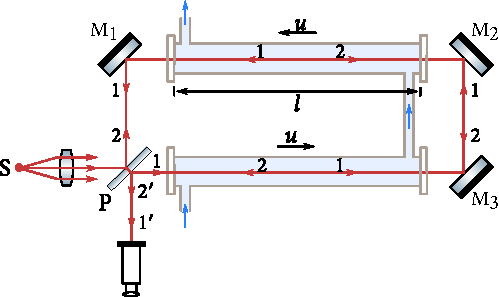
\includegraphics[scale=1]{figures/ch_21/fig_21_3.pdf}
		% \caption[]{}
        \caption[]{Fizeau's interferometer experiment to determine the role of the ether in the motion bodies in it. A parallel beam of light from source S was split by half-silvered plate P into two beams $1$ and $2$.}
		\label{fig:21_3}
	\end{center}
	\vspace{-0.8cm}
\end{figure}

When the water was stationary, beams $1$ and $2$ covered the path $L$ in the same time.
If water in its motion even partly carries along ether, then when the flow of the water was switched on, ray $2$, which propagates opposite to the flow, would spend more time to cover the path $L$ than ray $1$ travelling in the direction of flow.
As a result, a certain path difference will appear between the rays, and the interference pattern will be displaced.

The path difference we are interested in appears only in the path of the rays in the water.
This path has the length $2l$.
Let the velocity of light in the water relative to the ether be $v$.
When ether is not carried along by the water, the speed of light relative to the arrangement will coincide with $v$.
Let us assume that the water in its motion partly carries along the ether, imparting to it the velocity $\alpha u$ relative to the arrangement ($u$ is the velocity of the water, and $\alpha$ is the drag coefficient).
Hence, the velocity of light relative to the arrangement will be $v+\alpha u$ for ray $1$ and $v-\alpha u$ for ray $2$.
Ray $1$ covers the path $2l$ during the time $t_1=2l/(v+\alpha u)$, and ray $2$ during the time $t_2=2l/(v-\alpha u)$.
It can be seen from \eqn{16_54} that the optical length of a path to cover which the time $t$ is required equals $ct$.
Hence, the path difference of rays $1$ and $2$ is $\delta=c(t_2-t_1)$.
Dividing $\delta$ by $\Delta$ by $\lambda_0$, we get the number of fringes by which the interference pattern will be displaced when the flow of water is switched on:
\begin{equation*}
	\Delta{N} = \frac{c(t_2-t_1)}{\lambda_0} = \frac{c}{\lambda_0} \parenthesis{\frac{2l}{v-\alpha u} - \frac{2l}{v+\alpha u}} = \frac{4cl\alpha u}{\lambda_0 (v^2 - \alpha^2 u^2)}.
\end{equation*}

Fizeau discovered that the interference fringes are indeed displaced.
The value of the drag coefficient corresponding to this displacement was
\begin{equation}\label{eq:21_3}
	\alpha = 1 - \frac{1}{n^2},
\end{equation}

\noindent
where $n$ is the refractive index of water.
Thus, Fizeau's experiment showed that ether (if it exists) is carried along by moving water only partly.

It is easy to see that the result of Fizeau's experiment is explained by the relativistic law of velocity addition.
According to the first of equations (8.27) in Vol. I, the velocities $v_x$ and $v_x'$ of a body in frames K and K$'$ are related by the expression
\begin{equation}\label{eq:21_4}
	v_x = \frac{v_x' + v_0}{1 + v_0 v_x'/c^2}
\end{equation}

\noindent
($v_0$ is the velocity of the frame K$'$ relative to the frame K).

Let us relate the reference frame K to Fizeau's instrument, and the frame K$'$ to the moving water.
Now, the part of $v_0$ will be played by the velocity of the water $u$, that of $v_x'$ by the velocity of the light relative to the water equal to $c/n$, and, finally, the part of $v_x$ will be played by the velocity of the light relative to the instrument $\ab{v}{inst}$.
Introduction of these values into \eqn{21_4} yields
\begin{equation*}
	\ab{v}{inst} = \frac{c/n + u}{1 + u(c/n)c^2} = \frac{(c/n) + u}{1 + u/(cn)}.
\end{equation*}

\noindent
The velocity of the water $u$ is much smaller than $c$.
The expression obtained can therefore be simplified as follows:
\begin{equation}\label{eq:21_5}
	\ab{v}{inst} = \frac{(c/n) + u}{1 + u/(cn)} = \approx \parenthesis{\frac{c}{n}+u} \parenthesis{1 - \frac{u}{cn}} \approx \frac{c}{n} + u \parenthesis{1 - \frac{1}{n^2}}
\end{equation}

\noindent
[we have disregarded the term $u^2/(cn)$].

According to classical notions, the velocity of light relative to the instrument $\ab{v}{inst}$ equals the sum of the velocity of light relative to ether, \ie, $c/n$, and of the velocity of ether relative to the instrument, \ie, $\alpha u$:
\begin{equation*}
	\ab{v}{inst} = \frac{c}{n} + \alpha u.
\end{equation*}

\noindent
A comparison with \eqn{21_5} gives the value obtained by Fizeau for the drag coefficient $\alpha$ [see \eqn{21_3}].

It must be borne in mind that only the velocity of light in a vacuum is the same in all reference frames.
Its velocity in a substance differs in different reference frames.
It has the value $c/n$ in the frame associated with the medium in which the light is propagating.

\section{Michelson's Experiment}\label{sec:21_3}

In 1881, Michelson carried out his famous experiment by means of which he counted on detecting the motion of the Earth relative to ether (the ether wind).
In 1887, he repeated his experiment together with Morley on an improved instrument.
The arrangement used by Michelson and Morley is shown in \fig{21_4}.
A brick foundation supported an annular iron trough with mercury.
A wooden float having the shape of the bottom half of a longitudinally cut doughnut floated on the mercury.
The float carried a massive square stone slab.
This design made it possible to smoothly turn the slab about the vertical axis of the arrangement.
A Michelson interferometer (see \fig{17_6}) was installed on the slab.
The interferometer was modified so that both rays before returning to the half-silvered plate cover a distance coinciding with the diagonal of the slab several times.
A diagram of the path of the rays is shown in \fig{21_5}.
The symbols in this figure correspond to those used in \fig{17_16}.

\begin{figure}[t]
	\begin{center}
		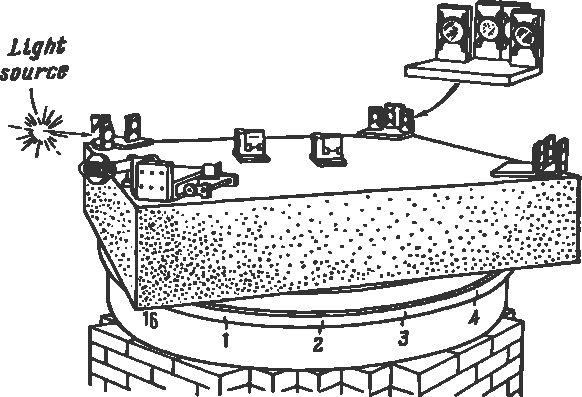
\includegraphics[scale=1]{figures/ch_21/fig_21_4.pdf}
		% \caption[]{}
        \caption[]{Michelson and Morley experiment. A brick foundation supported an annular iron trough with mercury. A wooden float having the shape of the bottom half of a longitudinally cut doughnut floated on the mercury. The float carried a massive square stone slab. This design made it possible to smoothly turn the slab about the vertical axis of the arrangement.}
		\label{fig:21_4}
	\end{center}
	\vspace{-0.8cm}
\end{figure}

\begin{figure}[t]
	\begin{center}
		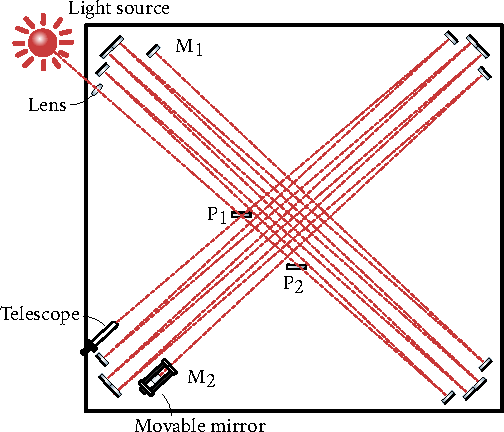
\includegraphics[scale=1]{figures/ch_21/fig_21_5.pdf}
		% \caption[]{}
        \caption[]{Modified Michelson interferometer. The interferometer was modified so that both rays before returning to the half-silvered plate cover a distance coinciding with the diagonal of the slab several times. The symbols in this figure correspond to those used in \fig{17_16}.}
		\label{fig:21_5}
	\end{center}
	\vspace{-0.8cm}
\end{figure}

The experiment was based on the following reasoning. Let us assume that interferometer arm PM$_2$ (\fig{21_6}) coincides with the direction of motion of the Earth relative to ether.
Consequently, the time needed for ray $1$ to cover the path to mirror M$_1$ and back will differ from the time needed for ray $2$ to cover path PM$_2$P.
As a result, even when the lengths of both arms are equal, rays $1$ and $2$ will acquire a certain path difference.
If we turn the arrangement through \ang{90}, the arms will exchange places, and the path difference will change its sign.
This should result in displacement of the interference pattern whose magnitude, as shown by calculations performed by Michelson, could be detected quite readily.

\begin{figure}[t]
	\begin{minipage}[t]{0.6\linewidth}
		\begin{center}
			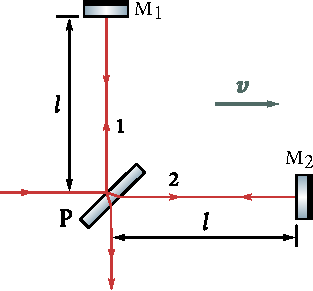
\includegraphics[scale=1]{figures/ch_21/fig_21_6.pdf}
			% \caption[]{}
            \caption[]{Reasoning of Michelson and Morley experiment, assuming that the interferometer arm PM$_2$ coincides with the direction of motion of the Earth relative to ether. Then, the time needed for ray $1$ to cover the path to mirror M$_1$ and back will differ from the time needed for ray $2$ to cover path PM$_2$P. As a result, even when the lengths of both arms are equal, rays $1$ and $2$ will acquire a certain path difference.
			Turning the arrangement \ang{90}, the arms will exchange places, and the path difference will change its sign.}
			\label{fig:21_6}
		\end{center}
	\end{minipage}
	\hfill{ }%space{-0.05cm}
	\begin{minipage}[t]{0.36\linewidth}
		\begin{center}
			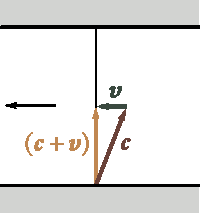
\includegraphics[scale=1]{figures/ch_21/fig_21_7.pdf}
            % \caption[]{}
			\caption[]{Considerations to calculate time $t_1$. Suppose that a launch developing the velocity $c$ relative to water has to cross a river with a current velocity of $v$ in a direction strictly perpendicular to its banks. For the launch to travel in the required direction, its velocity $c$ relative to the water must be directed as shown here.}
			\label{fig:21_7}
		\end{center}
	\end{minipage}
\vspace{-0.4cm}
\end{figure}

To calculate the expected displacement of the interference pattern, let us find the time spent by rays $1$ and $2$ to cover the relevant paths.
Assume that the Earth's velocity relative to the ether is $v$.
If the ether is not carried along by the Earth and the velocity of light relative to the ether is $c$ (the refractive index of air is practically equal to unity), then the velocity of light relative to the instrument will be $c - v$ for direction PM$_2$ and $c + v$ for direction M$_2$P.
Hence, the time needed for ray $2$ is determined by the expression
\begin{equation}\label{eq:21_6}
	t_2 = \frac{l}{c-v} + \frac{l}{c+v} = \frac{2lc}{c^2-v^2} = \frac{2l}{c} \frac{1}{(1-v^2/c^2)} \approx \frac{2l}{c} \parenthesis{1 + \frac{v^2}{c^2}}
\end{equation}

\noindent
(the Earth's velocity along its orbit is \SI{30}{km.s^{-1}}, therefore, $v^2/c^2= \num{e-8}\ll 1$).

Before commencing to calculate the time $t_1$, let us consider the following example from mechanics.
Suppose that a launch developing the velocity $c$ relative to water has to cross a river with a current velocity of $v$ in a direction strictly perpendicular to its banks (\fig{21_7}).
For the launch to travel in the required direction, its velocity $c$ relative to the water must be directed as shown in the figure.
Therefore, the velocity of the launch relative to the banks will be $|c+v|=\sqrt{c^2-v^2}$.
The velocity of ray $1$ relative to the arrangement (as assumed by Michelson) will be the same.
Consequently, the time taken by ray 1 is\footnote{We have used the formulas $\sqrt{1- x}\approx 1-x/2$ and $1/(1-x) \approx 1+x$, for small values of $x$.}
\begin{equation}\label{eq:21_7}
	t_1 = \frac{2l}{\sqrt{c^2-v^2}} = \frac{2l}{c} \frac{1}{\sqrt{1-v^2/c^2}} \approx \frac{2l}{c} \parenthesis{1 + \frac{1}{2} \frac{v^2}{c^2}}.
\end{equation}

Substituting for $t_2$ and $t_1$ in the expression $\Delta=c(t_2 - t_1)$ their values from expressions \eqref{eq:21_6} and \eqref{eq:21_7}, we get the path difference for rays $1$ and $2$:
\begin{equation*}
	\Delta = 2l \bracket{\parenthesis{1+\frac{v^2}{c^2}} - \parenthesis{1 + \frac{1}{2} \frac{v^2}{c^2}}} = l \frac{v^2}{c^2}.
\end{equation*}

\noindent
When the arrangement is turned through \ang{90}, the path difference changes its sign.
Consequently, the number of fringes by which the interference pattern will be displaced is
\begin{equation}\label{eq:21_8}
	\Delta{N} = \frac{2\Delta}{\lambda_0} = 2 \frac{l}{\lambda_0} \frac{v^2}{c}.
\end{equation}

The arm length $l$ (taking into account multifold reflections) was \SI{11}{m}.
The wavelength of the light used by Michelson and Morley was \SI{0.59}{\micro\metre}.
The use of these values in \eqn{21_8} gives
\begin{equation*}
	\Delta{N} = \frac{2\times 11}{\num{0.59e-6}} \times \num{e-8} = 0.37 \approx 0.4\text{ fringe}.
\end{equation*}

\noindent
The arrangement made it possible to detect a displacement of the order of $0.01$ fringe.
But no displacement of the interference pattern was detected.
The experiment was repeated during different times of the day to exclude the possibility of the horizon plane being perpendicular to the vector of the Earth's orbital velocity at the moment of measurements.
Subsequently, the experiment was repeated many times during different seasons of the year (during a year, the vector of the Earth's orbital velocity turns in space through \ang{360}), and negative results were constantly obtained.
The attempt to detect an ether wind was not successful Universal ether remained elusive.

Several attempts were made to explain the negative result of Michelson's experiment without refuting the hypothesis of the existence
of universal ether.
But all these attempts were groundless.
An exhaustive non-contradictory explanation of all the experimental facts including the results of Michelson's experiment was given by Albert Einstein in 1905.
He arrived at the conclusion that universal ether, \ie, a special medium that could serve as an absolute reference frame, does not exist.
Accordingly, Einstein extended the mechanical principle of relativity to all physical phenomena without any exception.
He further postulated in accordance with experimental data that the speed of light in a vacuum is the same in all inertial reference frames and does not depend on the motion of the light sources and receivers.

The principle of relativity and the principle of the constancy of the speed of light form the foundation of the special theory of relativity developed by Einstein (see Chapter 8 of Vol. I).

\section{The Doppler Effect}\label{sec:21_4}

In acoustics, the change in frequency due to the Doppler effect is determined by the velocities of the source and the receiver relative to the medium that is the carrier of the sound waves [see \eqn{14_78}].
The Doppler effect also exists for light waves.
But there is no special medium that would serve as the carrier of electromagnetic waves.
Therefore, the Doppler displacement of the frequency of light waves is determined only by the relative velocity of the source and the receiver.

Let us associate the origin of coordinates of the frame K with a light source and the origin of coordinates of the frame K$'$ with a receiver (\fig{21_8}).
We shall direct the axes $x$ and $x'$, as usual, along the velocity vector $v$ with which the frame K$'$ (\ie, the receiver) is moving relative to the frame K (\ie, the source).
The equation of a plane light wave emitted by the source in the direction of the receiver will have the following form in the frame K:
\begin{equation}\label{eq:21_9}
	E(x,t) = A \cos\bracket{\omega \parenthesis{t - \frac{x}{c}} + \alpha}.
\end{equation}

\noindent
Here, $\omega$ is the frequency of a wave registered in the reference frame associated with the source, \ie, the frequency of oscillations of the source.
We assume that the light wave is propagating in a vacuum; therefore, the phase velocity is $c$.

\begin{figure}[t]
	\begin{center}
		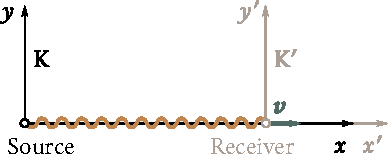
\includegraphics[scale=1]{figures/ch_21/fig_21_8.pdf}
		% \caption[]{}
        \caption[]{The Doppler effect for light waves. Let us associate the origin of coordinates of the frame K with a light source and the origin of coordinates of the frame K$'$ with a receiver. We shall direct the axes $x$ and $x'$, along the velocity vector $v$ with which the frame K$'$ (the receiver) is moving relative to the frame K (the source).}
		\label{fig:21_8}
	\end{center}
	\vspace{-0.8cm}
\end{figure}

According to the principle of relativity, the laws of nature have the same form in all inertial reference frames.
Hence, in the frame K$'$, the wave given by \eqn{21_9} will be described by the equation
\begin{equation}\label{eq:21_10}
	E(x',t') = A' \cos\bracket{\omega' \parenthesis{t' - \frac{x'}{c}} + \alpha'},
\end{equation}

\noindent
where $\omega'$ is the frequency registered in the reference frame K$'$, \ie, the frequency picked up by the receiver.
We have provided all the quantities except $c$, which is the same in all reference frames, with primes.

We can obtain an equation of a wave in the frame K$'$ from an equation in the frame K by passing over from $x$ and $t$ to $x'$ and $t'$ with the aid of the Lorentz transformations.
Introducing instead of $x$ and $t$ in \eqn{21_9} their values in accordance with Eqs. (8.17) of Vol. I, we get
\begin{equation*}
	E(x',t') = A\cos\bracket{\omega \parenthesis{ \frac{t'+(v/c^2)x'}{\sqrt{1-v^2/c^2}} - \frac{x'+vt'}{c \sqrt{1-v^2/c^2}} } +\alpha }
\end{equation*}

\noindent
(the part of $v_0$ is played by $v$).
The latter expression is easily transformed into the following one:
\begin{equation}\label{eq:21_11}
	E(x',t') = A\cos\bracket{\omega \parenthesis{ \frac{1-v/c}{\sqrt{1-v^2/c^2}} } \parenthesis{t' - \frac{x'}{c}} +\alpha }.
\end{equation}

Equation \eqref{eq:21_11} describes the same wave in the frame K$'$ as \eqn{21_10}.
Therefore, the following relation must be observed:
\begin{equation*}
	\omega' = \omega \frac{1-v/c}{\sqrt{1-v^2/c^2}} = \omega \parenthesis{\frac{1-v/c}{1+v/c}}^{1/2}.
\end{equation*}

\noindent
Let us change our notation: we shall denote the frequency $\omega$ of the source by $\omega_0$, and the frequency $\omega'$ of the receiver by $\omega$.
The preceding equation will thus become
\begin{equation}\label{eq:21_12}
	\omega = \omega_0 \parenthesis{\frac{1-v/c}{1+v/c}}^{1/2}.
\end{equation}

\noindent
Passing over from the angular frequency to the ordinary one, we have
\begin{equation}\label{eq:21_13}
	\nu = \nu_0 \parenthesis{\frac{1-v/c}{1+v/c}}^{1/2}.
\end{equation}

The velocity $v$ of the receiver relative to the source in \eqns{21_12}{21_13} is an algebraic quantity.
When the receiver moves away from the source, $v > 0$, and by \eqn{21_12}, $\omega<\omega_0$; when the receiver approaches the source, $v<0$, so that $\omega>\omega_0$.
When $v\ll c$, \eqn{21_12} can be written approximately as follows:
\begin{equation*}
	\omega \approx \omega_0 \bracket{ \frac{1 -(1/2)(v/c)}{1 + (1/2)(v/c)} } \approx \omega_0 \parenthesis{1 - \frac{1}{2} \frac{v}{c}} \parenthesis{1 - \frac{1}{2} \frac{v}{c}}.
\end{equation*}

\noindent
Hence, after Taylor expansion around $v=0$ and limiting ourselves to terms of the order of $v/c$, we get
\begin{equation}\label{eq:21_14}
	\omega = \omega_0 \parenthesis{1 - \frac{v}{c}}.
\end{equation}

\noindent
From this formula, we can find the relative change in the frequency:
\begin{equation}\label{eq:21_15}
	\frac{\Delta{\omega}}{\omega} = - \frac{v}{c}
\end{equation}

\noindent
($\Delta{\omega}$ stands for $\omega-\omega_o$).

We can show that a \textbf{transverse Doppler effect} exists for light waves in addition to the longitudinal effect we have considered.
It consists in a reduction in the frequency picked up by the receiver observed when the vector of the relative velocity is directed at right angles to the straight line passing through the receiver and the source\footnote{We remind our reader that the transverse Doppler effect does not exist for sound waves.} (when, for example, the source travels along a circle at whose centre the receiver is).
In this case, the frequency $\omega_0$ in the frame of the source is associated with the frequency $\omega$ in the frame of the receiver by the relation
\begin{equation}\label{eq:21_16}
	\omega = \omega_0 \parenthesis{1 - \frac{v^2}{c^2}}^{1/2} \approx \omega_0 \parenthesis{1 - \frac{1}{2} \frac{v^2}{c^2}}.
\end{equation}

The relative change in frequency in the transverse Doppler effect
\begin{equation}\label{eq:21_17}
	\frac{\Delta{\omega}}{\omega} = - \frac{1}{2} \frac{v^2}{c^2},
\end{equation}

\noindent
is proportional to the square of the ratio $v/c$ and, consequently, is considerably smaller than in the longitudinal effect for which the
relative change in the frequency is proportional to the first power of $v/c$.

The existence of the transverse Doppler effect was proved experimentally by the American physicist Herbert Ives (1882-1953) in 1938.
He determined the change in the frequency of emission of hydrogen atoms in canal rays (see the last paragraph of \sect{12_6}).

The velocity of the atoms was about \SI{2e8}{m.s^{-1}}.
These experiments were a direct experimental confirmation of the correctness of Lorentz transformations.

In the general case, the vector of the relative velocity can be resolved into two components of which one is directed along the ray, and the other at right angles to it.
The first component gives rise to the longitudinal, and the second to the transverse Doppler effect.

The longitudinal Doppler effect is used to determine the radial velocity of stars.
By measuring the relative shift of the lines in the spectra of stars, we can use \eqn{21_12} to determine $v$.

The thermal motion of the molecules of a luminous gas, owing to the Doppler effect, leads to broadening of the spectral lines.
As a result of the chaotic nature of the thermal motion, all the directions of the molecules' velocities relative to a spectrograph are equally probable.
Therefore, the radiation registered by the instrument contains all the frequencies in the interval from $\omega_0(1 - v/c)$ to $\omega_o (1 + v/c)$, where $\omega_0$ is the frequency emitted by the molecules, and $v$ is the velocity of thermal motion [see \eqn{21_14}].
The registered width of a spectral line is thus $2\omega_0v/c$.
The quantity
\begin{equation}\label{eq:21_18}
	\delta{\ab{\omega}{D}} = 2\omega_0 \frac{v}{c},
\end{equation}

\noindent
is called the \textbf{Doppler width of a spectral line} ($v$ stands for the most probable velocity of the molecules).
The magnitude of the Doppler broadening of spectral lines makes it possible to assess the velocity of thermal motion of the molecules and, consequently, the temperature of a luminous gas.
